\begin{frame}

\frametitle{The IEEE-754 Standard for Floating-Point Arithmetic}

\vspace{\fill}

\begin{center}

The standard way to deal with non-integral numbers on a \\ computer (i.e.,
numbers having fractional parts).

\vspace{\fill}

A tradeoff between speed, accuracy, dynamic range, \\ ease of use, and ease of
implementation.

\end{center}

\vspace{\fill}

\begin{itemize}

\item Established in 1985, revised in 2008.

\item Supported in hardware, so also the most efficient way.

\item Sometimes, computer performance is even measured in \\ terms of FLOPS
(Floating-Point Operations Per Second).

\end{itemize}

\end{frame}


\begin{frame}

\frametitle{Bad Computer Arithmetic Can Be Catastrophic}

\begin{center}

\vspace{\fill}

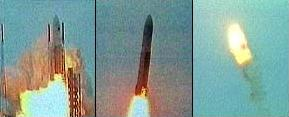
\includegraphics[scale=0.5]{figures/explosion.jpg}

\vspace{\fill}

The Ariane 5 rocket (1996) exploded seconds after lift-off \\ due a mixture of
arithmetical and logical errors \\ in the inertial navigation system.

\vspace{\fill}

The rocket and is cargo were valued at 500 million USD.

\end{center}

\end{frame}


\begin{frame}

\frametitle{Where You Might Have Met IEEE-754}

\vspace{\fill}

\begin{tabular}{ll}
\multicolumn{2}{l}{\textbf{R}} \\
\texttt{numeric} & IEEE-754 Double Precision Floating-Point \\
\multicolumn{2}{l}{\textbf{Python}} \\
\texttt{float} &  IEEE-754 Double Precision Floating-Point \\
\multicolumn{2}{l}{\textbf{Matlab}} \\
\texttt{single} & IEEE-754 Single Precision Floating-Point \\
\texttt{double} & IEEE-754 Double Precision Floating-Point \\
\multicolumn{2}{l}{\textbf{Excel}} \\
\texttt{SINGLE} & IEEE-754 Single Precision Floating-Point \\
\texttt{DOUBLE} & IEEE-754 Double Precision Floating-Point
\end{tabular}

\vspace{\fill}

\end{frame}

\begin{frame}

\vspace{\fill}

\begin{center}

\huge \textbf{How did we get here?}

\vspace{0.5in}

\large How does the IEEE-754 standard work and why?

\end{center}

\vspace{\fill}

\end{frame}
